%% Manuscript for International Transactions in Operational Research (ITOR),
%% prepared with the ITOR class (itor.cls, v1.0). Every number comes from
%% generated macros or generated tables (code/itor_tables.py).
\documentclass{itor}

\usepackage{natbib}
\usepackage{url}
\urlstyle{same}
\usepackage{amsmath,amssymb,booktabs,array}
\usepackage{xr-hyper}
\usepackage[hidelinks]{hyperref}
\externaldocument[S-]{si_labels}
\newcommand{\SI}[1]{Section~\ref{S-#1}}
\providecommand{\bibcommenthead}{}

\newcommand{\ProcConsRange}{8.3--21.4}
\newcommand{\ConservativeSelected}{25}
\newcommand{\ConservativeRetained}{25}
\newcommand{\CappedSelected}{42}
\newcommand{\CappedRetained}{40}
\newcommand{\OriginalRetained}{30}
\newcommand{\OriginalProbability}{78.9}
\newcommand{\ConservativeProbability}{78.6}
\newcommand{\CappedProbability}{86.6}
\newcommand{\ClockFound}{49}
\newcommand{\CappedGainInterval}{7.7 [3.5, 12.5]}
\newcommand{\CappedDistanceCost}{2.5}
\newcommand{\CappedFleetCost}{0.43}
\newcommand{\OriginalSelected}{32}
\newcommand{\FailureCount}{21}
\newcommand{\CertifiedFailures}{17}
\newcommand{\SweepLowIndep}{-3.1}
\newcommand{\SweepHighIndep}{30.5}
\newcommand{\CappedLargeRange}{97.5--97.6}
\newcommand{\CappedLargeSelected}{18/18}
\newcommand{\CappedLargeRetained}{16/18}
\newcommand{\OriginalSelectedMean}{97.3}
\newcommand{\OriginalFallbackMean}{50.9}
\newcommand{\CappedSelectedMean}{97.4}
\newcommand{\CappedFallbackMean}{45.2}
\newcommand{\CappedFallbackCount}{11}
\newcommand{\BudgetDiagCases}{8}
\newcommand{\BudgetDiagSearchLimits}{4}
\newcommand{\BudgetDiagUnresolved}{4}
\newcommand{\CappedFleetLarge}{1.88}
\newcommand{\ConfInstances}{53}
\newcommand{\ConfCommon}{50}
\newcommand{\ConfHOneMean}{15.7}
\newcommand{\ConfHOneLo}{7.5}
\newcommand{\ConfHOneHi}{23.6}
\newcommand{\ConfHTwoMean}{11.7}
\newcommand{\ConfHTwoLo}{5.9}
\newcommand{\ConfHTwoHi}{17.9}
\newcommand{\ConfHThreeK}{46}
\newcommand{\ConfHThreeP}{32}
\newcommand{\ConfHThreeKonly}{14}
\newcommand{\ConfHThreePonly}{0}
\newcommand{\ConfHThreeExact}{0.00012}
\newcommand{\ConfHFourMean}{28.3}
\newcommand{\ConfHFourLo}{19.6}
\newcommand{\ConfHFourHi}{36.4}
\newcommand{\ConfPooledP}{79.4}
\newcommand{\ConfPooledSC}{82.4}
\newcommand{\ConfPooledK}{91.0}
\newcommand{\ConfRetainedP}{31/32}
\newcommand{\ConfRetainedK}{45/46}
\newcommand{\ConfNoPlanConservative}{3}
\newcommand{\ConfNoPlanClock}{4}
\newcommand{\ConfAdmMeanP}{97.4}
\newcommand{\ConfFbMeanP}{51.9}
\newcommand{\ConfFbCountP}{21}
\newcommand{\ConfAdmMeanK}{97.5}
\newcommand{\ConfFbMeanK}{48.7}
\newcommand{\ConfFbCountK}{7}
\newcommand{\PostHocP}{85.0}
\newcommand{\PostHocK}{93.0}
\newcommand{\PostHocChangedP}{18}
\newcommand{\PostHocChangedK}{6}
\newcommand{\HTwoFromKonly}{11.6}
\newcommand{\WtEqualDiffMean}{$-$8.8}
\newcommand{\WtEqualDiffLo}{$-$14.3}
\newcommand{\WtEqualDiffHi}{$-$3.5}
\newcommand{\WtEqualPCMean}{6.3}
\newcommand{\WtEqualPCLo}{$-$1.1}
\newcommand{\WtEqualPCHi}{13.7}
\newcommand{\WtEqualAdmitted}{23}
\newcommand{\WtBaseAdmitted}{31}
\newcommand{\WtDistanceHeavyPCMean}{12.7}
\newcommand{\WtDistanceHeavyPCLo}{5.3}
\newcommand{\WtDistanceHeavyPCHi}{19.7}
\newcommand{\SolomonN}{8}
\newcommand{\SolomonPlans}{5}
\newcommand{\SolomonAdmitted}{3}
\newcommand{\SolomonNoPlan}{3}

\newcommand{\CtwoGOneMean}{28.0}
\newcommand{\CtwoGOneLo}{23.0}
\newcommand{\CtwoGOneHi}{32.8}
\newcommand{\CtwoGTwoMean}{0.4}
\newcommand{\CtwoGTwoLo}{$-$0.7}
\newcommand{\CtwoGTwoHi}{2.1}
\newcommand{\CtwoGThreeMean}{3.8}
\newcommand{\CtwoGThreeLo}{1.6}
\newcommand{\CtwoGThreeHi}{6.2}
\newcommand{\CtwoGFourMean}{$-$0.2}
\newcommand{\CtwoGFourLo}{$-$4.0}
\newcommand{\CtwoGFourHi}{3.7}
\newcommand{\CtwoCommon}{49}
\newcommand{\CtwoPooledHGSCons}{58.4}
\newcommand{\CtwoPooledHGSK}{91.6}
\newcommand{\CtwoPooledORTK}{91.4}
\newcommand{\CtwoPooledORTKc}{91.7}
\newcommand{\CtwoORTKAdmitted}{45}
\newcommand{\CtwoORTKFallbacks}{8}
\newcommand{\CtwoFallbacksChanged}{4}
\newcommand{\CtwoHGSKAdmittedLarge}{18}
\newcommand{\CtwoHGSPAdmittedLarge}{3}
\newcommand{\CtwoLarge}{18}
\newcommand{\DevHGSGOneMean}{27.0}
\newcommand{\DevHGSGOneLo}{23.0}
\newcommand{\DevHGSGOneHi}{30.8}
\newcommand{\DevHGSPooledK}{94.2}

\newcommand{\RobInstances}{45}
\newcommand{\RobNoPlanBoxFour}{8}
\newcommand{\RobNoPlanBoxSix}{16}
\newcommand{\RobBoxFourP}{75.0}
\newcommand{\RobBoxSixP}{63.3}
\newcommand{\RobCapGThreeFourP}{89.4}
\newcommand{\RobCapBoxFourP}{91.4}
\newcommand{\RobCapGThreeSixP}{97.8}
\newcommand{\RobCapBoxSixP}{98.4}
\newcommand{\RobScreenedP}{87.4}
\newcommand{\RobScreenedCapP}{97.2}
\newcommand{\RobScreenedCapAdm}{44}
\newcommand{\RobScreenedAdm}{29}
\newcommand{\RobOrtCappedP}{84.6}
\newcommand{\RobHgsCappedP}{93.6}
\newcommand{\RobOrtNominalD}{1.7}
\newcommand{\RobReliefGain}{16.4}
\newcommand{\RobCapGThreeFourMinusOrt}{4.8}
\newcommand{\RobCapGThreeFourMinusOrtLo}{$-$1.4}
\newcommand{\RobCapGThreeFourMinusOrtHi}{11.6}
\newcommand{\RobCapGThreeFourMinusOrtFleet}{0.42}
\newcommand{\RobCapGThreeSixMinusHgs}{4.2}
\newcommand{\RobCapGThreeSixMinusHgsLo}{1.3}
\newcommand{\RobCapGThreeSixMinusHgsHi}{7.7}
\newcommand{\RobCapGThreeSixMinusHgsFleet}{0.67}
\newcommand{\RobScreenedCapMinusHgs}{3.6}
\newcommand{\RobScreenedCapMinusHgsLo}{0.6}
\newcommand{\RobScreenedCapMinusHgsHi}{7.1}
\newcommand{\RobScreenedCapMinusHgsFleet}{0.53}
\newcommand{\RobBenchEqualTwenty}{20}
\newcommand{\RobBenchCountTwenty}{20}
\newcommand{\RobBenchGapFifty}{0.04}
\newcommand{\RobBenchGapHundred}{0.9}
\newcommand{\RobItersSmall}{6000}
\newcommand{\RobItersHundred}{3000}

\newcommand{\FwAdmittedOrig}{318}
\newcommand{\FwAdmittedTotal}{306}
\newcommand{\FwMissOrig}{11}
\newcommand{\FwMissFw}{1}
\newcommand{\FwLostMax}{2}
\newcommand{\FwPooledChangeMin}{$-$1.8}
\newcommand{\FwPooledChangeMax}{0.2}
\newcommand{\FwAdmMeanMin}{97.7}
\newcommand{\FwAdmMeanMax}{98.3}
\newcommand{\AdmMeanMin}{97.3}
\newcommand{\AdmMeanMax}{98.0}
\newcommand{\TimeScreenTwenty}{3}
\newcommand{\TimeScreenTwoHundred}{24}
\newcommand{\TimeHgsTwenty}{2.2}
\newcommand{\TimeHgsTwoHundred}{9.3}
\newcommand{\BetaOrtMid}{191}
\newcommand{\BetaOrtN}{225}
\newcommand{\BetaOrtEdge}{4}
\newcommand{\BetaHgsEdge}{11}
\newcommand{\BetaHgsN}{93}
\newcommand{\MisMinOrig}{11.5}
\newcommand{\MisMinOrt}{21.9}
\newcommand{\MisMinHgs}{23.3}
\newcommand{\MisCappedDrop}{6.9}
\newcommand{\MisConsDrop}{21.2}
\newcommand{\MisKOrt}{159}
\newcommand{\MisKHgs}{106}
\newcommand{\MisKRob}{45}

\newcommand{\FbGainMin}{3.0}
\newcommand{\FbGainMax}{15.6}
\newcommand{\FbCappedPooledMin}{95.1}
\newcommand{\FbCappedPooledMax}{97.2}
\newcommand{\PbFOne}{7.3}
\newcommand{\PbFOneLo}{2.3}
\newcommand{\PbFOneHi}{13.2}
\newcommand{\PbFTwo}{4.2}
\newcommand{\PbFTwoLo}{1.2}
\newcommand{\PbFTwoHi}{8.0}
\newcommand{\PbFThree}{94.4}
\newcommand{\PbFThreeLo}{90.1}
\newcommand{\PbFThreeHi}{97.1}
\newcommand{\PbFFour}{94.9}
\newcommand{\PbFFourLo}{91.0}
\newcommand{\PbFFourHi}{97.1}
\newcommand{\PbInstances}{53}
\newcommand{\PbOrtFallbacks}{9}
\newcommand{\PbHgsFallbacks}{8}
\newcommand{\PbOrtPooled}{87.1}
\newcommand{\PbHgsPooled}{90.7}
\newcommand{\PbNoAnchor}{1}
\newcommand{\PbExOrt}{96.3}
\newcommand{\PbExHgs}{96.7}
\newcommand{\PaROne}{6.7}
\newcommand{\PaROneLo}{3.0}
\newcommand{\PaROneHi}{11.1}
\newcommand{\PaRTwo}{6.7}
\newcommand{\PaRTwoLo}{2.2}
\newcommand{\PaRTwoHi}{12.2}
\newcommand{\PaRThree}{0.42}
\newcommand{\PaRFour}{$-$1.3}
\newcommand{\PaRFourAbs}{1.3}
\newcommand{\PaBoxMinusScr}{1.2}
\newcommand{\PaInstances}{90}
\newcommand{\PaScreenedP}{97.2}
\newcommand{\PaOrtP}{90.5}
\newcommand{\PaHgsP}{90.6}
\newcommand{\PaBoxP}{98.4}
\newcommand{\PaAdmitted}{86}
\newcommand{\FmHgs}{$-$1.9}
\newcommand{\FmHgsLo}{$-$5.1}
\newcommand{\FmHgsHi}{1.5}
\newcommand{\FmConfHgs}{3.2}
\newcommand{\FmConfHgsLo}{$-$1.1}
\newcommand{\FmConfHgsHi}{8.1}
\newcommand{\FmConfOrt}{$-$0.7}
\newcommand{\FmConfOrtLo}{$-$3.9}
\newcommand{\FmConfOrtHi}{2.7}
\newcommand{\BrOrigAdv}{17.5}
\newcommand{\BrEqAdv}{8.1}
\newcommand{\BrEqAdvLo}{1.1}
\newcommand{\BrEqAdvHi}{15.1}
\newcommand{\BrDurDiff}{$-$8.9}
\newcommand{\BrFleetDiff}{$-$5.6}
\newcommand{\BrEqDiff}{$-$8.5}
\newcommand{\GhAdmitted}{17}
\newcommand{\GhAttempted}{18}
\newcommand{\GhDiff}{15.1}
\newcommand{\GhDiffLo}{11.0}
\newcommand{\GhDiffHi}{19.1}
\newcommand{\GhCapped}{87.2}
\newcommand{\GhCons}{73.6}

\newcommand{\PaRThreeLo}{0.20}
\newcommand{\PaRThreeHi}{0.67}
\newcommand{\PaRFourLo}{$-$1.7}
\newcommand{\PaRFourHi}{$-$0.9}
\newcommand{\ItorCostDistRange}{2.0--4.9}


\jname{International Transactions in Operational Research}
\jvol{XX}
\jyear{20XX}
\doi{xx.xxxx/itor.xxxxx}

\begin{document}

\title{Reliability screening for vehicle routing with time windows: a
solver-independent alternative to travel-time padding}

\author[S. Ali]{Suhan Ali\affmark{a,$\ast$}}
\affil{\affmark{a}Independent researcher, Lahore, Pakistan}
\email{syedsuhanali9@gmail.com [S. Ali]}
\thanks{\affmark{$\ast$}Author to whom all correspondence should be addressed
(e-mail: syedsuhanali9@gmail.com). ORCID: 0009-0004-5079-7684.}

\historydate{Received DD MMMM YYYY; received in revised form DD MMMM YYYY; accepted DD MMMM YYYY}

\begin{abstract}
Routing plans built on nominal travel times fail under congestion and
random delay, and the usual safeguard of padding every trip wastes capacity on
safe routes. This paper adds a statistical reliability check
to any solver for the vehicle routing problem with time windows. The solver
generates candidate plans with internal buffers that leave customer windows
unchanged. A plan is admitted only if a 95\% Wilson lower bound on the
probability that at least 95\% of customers are served on time reaches 0.95;
admitted plans are validated on fresh scenarios. Capping each buffer at
the customer's direct-reachability limit removes a failure that also blocks
budgeted-robust models. On synthetic instances with 20--200 customers,
screening beat 20\% padding by \ProcConsRange{} percentage points (not
significant at 200 customers). In three timestamped protocols,
seven of eight primary hypotheses held; a conservative-speed fallback did
not measurably help. Results depend on the assumed delay model.
\end{abstract}

\keywords{vehicle routing; time windows; stochastic travel times; time-dependent
travel times; chance constraints; simulation; reproducibility}

\maketitle

\section{Introduction}

The vehicle routing problem with time windows (VRPTW) asks a fleet to serve
customers within agreed windows, subject to vehicle capacity and shift length
\citep{solomon1987,toth2014}. Most planning tools solve it on one fixed matrix
of travel times. Real travel times change with the time of day and with random
delays, and a delay early in a route pushes every later customer towards the end
of its window. A plan that is optimal on nominal times takes no account of this.

The simplest safeguard is to plan at a slower speed than expected. Padding every
trip by a fixed percentage is easy to explain and needs no new software, but it
protects off-peak trips as much as peak ones and adds distance and vehicles
whether or not a route is at risk. Stochastic and robust VRPTW models avoid that
waste by building the uncertainty into the optimization
\citep{errico2018,agra2013,gendreau2016}. They need a solver written for their
uncertainty model, and most operators run a general solver that they cannot
easily replace.

This paper studies a procedure that sits between the two. A standard VRPTW
solver proposes a family of candidate plans, each planned against internal
deadlines contracted by a buffer, while the windows promised to customers stay
fixed. Each candidate is simulated on a bank of scenarios drawn from a
time-dependent, correlated delay model, and it is admitted only if a one-sided
Wilson lower bound on the probability of a good service day reaches a target.
Among admitted plans the procedure returns the best under the planner's own
objective, and it reports that plan's reliability from an independent
validation bank that played no part in the choice. The solver and its objective
are left as they are; reliability is judged after the solve, by the same rule
for every solver.

The paper makes three contributions.
\begin{enumerate}
\item It specifies this screening-and-validation procedure and identifies a
failure that internal buffers create: a contracted deadline can make a customer
unreachable even by a direct trip, so the solver finds no plan. Capping each
customer's buffer at its direct-reachability limit removes that failure. The
same obstruction appears in a budgeted-robust VRPTW model, and the analogous
relief removes it there too.
\item It gives matched evidence on when screening beats uniform padding and at
what cost. In a development study on 53 synthetic instances with 20 to 200
customers, the screened procedure was \ProcConsRange{} percentage points more
reliable than 20\% padding, depending on size; at 200 customers the interval
included zero. Three protocols, each publicly timestamped with
frozen code before its runs \citep{ali2026freeze,ali2026freeze2,ali2026freeze3},
then tested the main findings on new instances, with OR-Tools \citep{ortools}
and hybrid genetic search (HGS; \citealp{vidal2022,wouda2024}) as generators.
Seven of their eight primary hypotheses met their decision criteria, and the
paper reports the one that did not.
\item It places the procedure against a budgeted-robust optimizer
\citep{bertsimas2004,agra2013} and tests a fallback rule for instances where no
plan passes. The robust plans with reachability relief, screened in the same
way, were more reliable on instances with up to 100 customers but used more
vehicles; restricted to the comparator's fleet, their advantage was no longer
measurable. Returning the best-screened candidate when nothing is admitted
raised pooled service in a prespecified test on 53 further instances.
\end{enumerate}

The instances are synthetic and the delay model is assumed, so the evidence
shows repeatability within one setting. Every number in the paper is regenerated
from the archived records, and the full model, every result table and further
checks are in the Supporting Information (SI).

Section~\ref{sec:related} reviews related work. Section~\ref{sec:method}
defines the planning model, the evaluation model and the procedure.
Section~\ref{sec:design} describes the experiments and
Section~\ref{sec:results} the results. Section~\ref{sec:discussion} discusses
implications and limitations, and Section~\ref{sec:conclusion} concludes.

\section{Related work}\label{sec:related}

Time-dependent routing needs care because a speed multiplier applied at
departure can break first-in-first-out (FIFO). \citet{ichoua2003} introduced
the integrated speed-profile construction used here, and \citet{ghiani2014}
analysed its properties. Stochastic VRPTW research treats uncertain travel and
service times through chance constraints, recourse, approximate feasibility
tests and data-driven formulations
\citep{laporte1992,kenyon2003,li2010,errico2018,bomboi2022,serrano2026}.
\citet{ehmke2015} embed per-customer service levels in a routing method;
\citet{tas2014} jointly model time dependence, stochastic travel and soft
windows; and \citet{bomboi2022} check route feasibility under correlated,
time-dependent travel times. \citet{jabali2015} introduced self-imposed time
windows, and \citet{vareias2019} assign windows under stochastic travel times
with per-customer chance constraints. These are the closest analogues of the
internal contraction used here, but both build the buffers into a dedicated
optimization and judge reliability customer by customer. Neither can be added to
an unmodified solver, and neither bounds the probability of a whole service day.

A second line builds the uncertainty into the optimization. \citet{agra2013}
solve a robust VRPTW over a budgeted uncertainty set \citep{bertsimas2004};
\citet{jaillet2016} minimize a requirements violation index; and
\citet{zhang2019} develop a riskiness index with an exact algorithm. Surveys by
\citet{gendreau1996} and \citet{gendreau2016} cover stochastic routing more
broadly. This paper compares the procedure with padding and with one budgeted
robust model; it does not compare it with a chance-constrained or
distributionally robust VRPTW solver.

This paper makes its statistical claim after the solve. It does not build a
feasibility approximation into a specialist search. It takes routes from
a replaceable nominal solver, searches a family of internal buffers on one
scenario bank and checks the chosen plan once on a held-out bank. Its service
event limits the share of late customers across the whole day, which is closer
to the plan-level risk measures of \citet{kenyon2003} than to per-customer
constraints. Windows offered to customers never change. Monte Carlo
approximations of chance constraints need a separate check of the chosen
solution \citep{ahmed2008}, which the validation bank provides, and the Wilson
bound is used because normal-approximation intervals behave poorly near one
\citep{wilson1927,brown2001}.

\section{Model and procedure}\label{sec:method}

\subsection{Planning model}

Let $N=\{0,1,\ldots,n\}$ be the nodes, with depot 0 and customers $C$, and let
$V$ be a homogeneous fleet with capacity $Q$ and maximum shift duration
$H^{\max}$. Customer $i$ has demand $\delta_i$, service time $s_i$ and offered
window $[l_i,u_i]$ for the start of service. Planning uses nominal distances
$d_{ij}$ and times $\bar t_{ij}$. A plan assigns customers to routes, fixes the
visit order and sets a depot departure $d_v$ and return $r_v$ for each vehicle
$v$, with service start $a_i$ at each customer. The full formulation is in
\SI{sec:si-model}; there $x_{ijv}=1$ if vehicle $v$ drives arc $(i,j)$ and
$y_v=1$ if vehicle $v$ is used. Four criteria describe a plan:
\begin{equation}
 F_1=c_f\sum_{v}\sum_{i,j}d_{ij}x_{ijv},\quad
 F_2=\sum_{i\in C}\max\{0,s^*-(u_i-a_i)\},\quad
 F_3=\sum_{v}(r_v-d_v),\quad
 F_4=\sum_{v}y_v,                                       \label{eq:criteria}
\end{equation}
namely distance cost at $c_f$ per kilometre, slack deficit against a target slack $s^*$, driver
duration and fleet use. Each criterion is scaled by the range $[L_k,U_k]$ it
takes over four single-criterion anchor solutions, and the candidate objective
is
\begin{equation}
 Z=\sum_{k=1}^{4}w_k\,\frac{F_k-L_k}{\max\{U_k-L_k,1\}}.        \label{eq:objective}
\end{equation}
The weights $\mathbf{w}=(0.5693,0.2643,0.1055,0.0609)$ are a fixed experimental
vector chosen before any experiment; their origin and a sensitivity analysis
are in \SI{sec:ahp-matrix} and Section~\ref{sec:checks}. The objective shapes the
candidates and ranks the admitted ones, but the admission test does not use it,
and any scalar objective could replace it.

\subsection{Evaluation model}

The day is split into periods $[T_k,T_{k+1})$ with speeds $\nu_k>0$. The
deterministic travel time from $i$ to $j$ when leaving at time $\tau$ is the
smallest $\Delta\geq0$ with
\begin{equation}
 \int_{\tau}^{\tau+\Delta}\nu(u)\,du=d_{ij},                 \label{eq:fifo}
\end{equation}
which preserves FIFO \citep{ichoua2003}. In scenario $\omega$ the realised
travel time is $t_{ij}(\tau)\exp\{\varepsilon_{ij}(\omega)\}$, with
\begin{equation}
 \varepsilon_{ij}(\omega)=\sigma\bigl(\sqrt{\rho}\,\xi_0(\omega)
 +\sqrt{1-\rho}\,\xi_{ij}(\omega)\bigr),                       \label{eq:noise}
\end{equation}
where $\xi_0$ is a common standard normal factor drawn once per scenario and
$\xi_{ij}$ is an arc-specific one. The multiplier has median one, so the
deterministic profile gives the median travel time. Each arc draws from its own
stream keyed by the bank seed and its endpoints, so plans evaluated on one bank
see the same disturbances on shared arcs. A fixed set of simulated days drawn in this way is called a scenario
\emph{bank}. Every vehicle leaves at its planned time in every scenario.

\subsection{Screening and validation}

For plan $R$ in scenario $\omega$, let $q(R,\omega)$ be the share of customers
whose service starts by $u_i$. The service event is
$J(R,\omega)=\mathbf{1}\{q(R,\omega)\geq\kappa\}$ with $\kappa=0.95$, and the
target is $\Pr[J=1]\geq\alpha$ with $\alpha=0.95$. Requiring every customer to
be on time would be a poor target for large instances, because that probability
falls with the number of customers even for good plans; it is reported but not
used for admission.

For each buffer $\beta$ in a grid, the solver plans against the contracted
deadline $\max\{l_i,u_i-\beta\}$ and minimizes~\eqref{eq:objective}, with the
anchor ranges fixed at their uncontracted values. Each candidate is simulated on
a screening bank of $N_s$ scenarios, and with empirical success $\hat p$ its
one-sided Wilson lower bound at level $1-\eta$ is
\begin{equation}
 L(\hat p)=\frac{\hat p+z^2/(2N_s)-z\sqrt{\hat p(1-\hat p)/N_s+z^2/(4N_s^2)}}{1+z^2/N_s},
 \qquad z=z_{1-\eta}.                                          \label{eq:wilson}
\end{equation}
A candidate is admitted when $L(\hat p)\geq\alpha$, and the admitted candidate
with the smallest $Z$ is selected. It is then simulated once on a larger,
untouched validation bank, which only reports its reliability. Scoring always
uses the offered windows $u_i$. If no candidate is admitted, a fallback rule
fixed in advance returns a plan, so the procedure has an output on every
instance. The results therefore distinguish the validated reliability of
admitted plans from the procedure-level reliability over all instances,
fallbacks included; the latter, averaged over instances, is called
\emph{pooled service}. The bound holds for each candidate separately; a
family-wise version over the grid is examined in Section~\ref{sec:checks}.
The procedure is:
\begin{enumerate}
\item For each buffer $\beta\in\{0,5,\ldots,60\}$ minutes, solve the planning
model with deadlines $\max\{l_i,u_i-\beta\}$ (or~\eqref{eq:cap} when capped).
\item Simulate each candidate on the screening bank and compute $L(\hat p)$.
\item If some candidate has $L(\hat p)\geq\alpha$, select the admitted
candidate with the smallest $Z$; otherwise apply the fallback rule.
\item Simulate the selected plan once on the validation bank and report its
service probability.
\end{enumerate}

\subsection{Reachability-capped contraction}

Contraction can make a customer unreachable even by a direct trip from the
depot, in which case no plan exists at that buffer. Let
$e_i=\max\{l_i,\bar t_{0i}\}$ be the earliest direct service time. The capped
procedure plans against
\begin{equation}
 u_i^{\rm cap}(\beta)=\min\bigl\{u_i,\max\{l_i,u_i-\beta,e_i\}\bigr\},
 \label{eq:cap}
\end{equation}
so contraction alone never removes a customer that was reachable before. The cap
does not guarantee that a joint routing exists or that the target is met. A
shortest-path relaxation certifies when a contracted model is infeasible, which
separates proven infeasibility from search failure (\SI{sec:capping}).

\subsection{Comparators}

\emph{Conservative speed} plans for distance at 33.3~km/h instead of 40~km/h,
which pads every trip by 20\%. \emph{Screened conservative speed} applies the
same screen to conservative-speed candidates. The \emph{original procedure}
screens contracted candidates without the cap, and the \emph{capped procedure}
uses~\eqref{eq:cap}. The candidate generator is OR-Tools \citep{ortools} or the
HGS of PyVRP \citep{wouda2024}, which solves the same planning model but cannot
express the slack-deficit term during generation.

The robust comparator is a VRPTW with budgeted uncertainty
\citep{bertsimas2004,agra2013}: on each arc the travel time may rise from
$\bar t_{ij}$ to $\bar t_{ij}+\lceil\theta\bar t_{ij}\rceil$, and a route must
stay feasible whenever at most $\Gamma$ of its arcs do so; \emph{box
uncertainty} is the case in which every arc may take its upper value. Feasibility is
checked exactly with the dynamic programme of \citet{agra2013} inside a large
neighbourhood search written for this study, which minimizes distance and stops
after a fixed number of iterations, so it is deterministic. Robust models meet
the same obstruction as contraction: a customer that cannot be reached on time
by a direct trip at its upper travel time makes every plan infeasible. The
\emph{relieved} variant raises such a customer's robust deadline to its
worst-case direct start while every original window must still hold under
nominal times. \emph{Screened robust} passes all robust plans of an instance
through the same screen and returns the shortest admitted one, or the one with
the highest screening success. \SI{sec:robust-design} gives the details.

Three fallback rules are compared: the uncontracted slack-aware plan
(\emph{slack-aware}), the generator's conservative-speed plan
(\emph{conservative}), and the candidate of the procedure's own family with the
highest screening success (\emph{best-screened}). None of them uses a validation
outcome. Unless stated otherwise, the OR-Tools procedures use the slack-aware
fallback and the HGS procedures the conservative one, as fixed in their
protocols.

\section{Experimental design}\label{sec:design}

Instances place a central depot and uniformly distributed customers on a
$100\times100$ grid. Demand is uniform on 10--49 units, service takes 10
minutes, window widths are uniform on 90--149 minutes, capacity is 1000 and the
shift lasts 600 minutes from 06:00. Table~\ref{tab:parameters} lists the
instance sizes and the model constants. The planned shift has a morning peak
from 07:00 to 09:00, and the speed profile continues into the evening so that
overrunning routes are still evaluated.

\begin{table}[t]
\centering
\footnotesize
\caption{Instances and parameters of the development study. The confirmatory
studies use the same sizes with the seeds shifted (Section~\ref{sec:design}).}
\label{tab:parameters}
\begin{tabular}{@{}p{0.43\textwidth}p{0.5\textwidth}@{}}
\toprule
Parameter & Value\\
\midrule
Customers (vehicles available; instances) & 20 (6; 20), 50 (14; 15), 100 (26; 10), 200 (40; 8)\\
Nominal speed; shift & 40~km/h; 600~min from 06:00\\
Speed divisors in the shift & 0.9 (06:00--07:00), 1.2 (07:00--09:00), 1.0 (09:00--16:00)\\
Capacity; service time; target slack $s^*$ & 1000; 10~min; 15~min\\
Disturbance $\sigma$; latent correlation $\rho$ & 0.20; 0.50 (sweep $\sigma\in\{0.1,0.2,0.3\}$, $\rho\in\{0,0.5,0.9\}$)\\
Service fraction $\kappa$; target $\alpha$; Wilson $\eta$ & 0.95; 0.95; 0.05 (one-sided)\\
Screening; validation; sweep scenarios & 1000; 5000; 1000 per cell\\
Buffer grid & $\beta\in\{0,5,\ldots,60\}$~min\\
Solver budgets & OR-Tools 5~s per candidate; HGS 10,000 iterations\\
\bottomrule
\end{tabular}
\end{table}

The development study ran every configuration on 53 instances with fixed seeds,
and its findings are exploratory. Within an instance all configurations share
the same screening and validation banks, so every comparison is paired.
Across-instance intervals use a paired bootstrap with 20,000 resamples and a
fixed seed. A configuration without a plan scores zero, so a failure counts
against the configuration that failed. Software errors are recorded and block
the analysis; they are never scored as routing outcomes.

Three confirmatory protocols followed. Each fixed its hypotheses, tests, decision
rules, failure policy and instance seeds, and was committed to a public
repository with a SHA-256 manifest of the code that runs and analyses it, and
archived on Zenodo, before any of its instances was solved
\citep{ali2026freeze,ali2026freeze2,ali2026freeze3}. The analysis programs stop
unless every record is present and every frozen file matches its manifest.
Protocol~1 tested the OR-Tools procedures on 53 new instances. Protocol~2 tested
HGS as the generator and the conservative fallback on 53 further instances.
Protocol~3 had two parts: part A repeated the robust comparison on the
\PaInstances{} confirmatory instances with up to 100 customers, and part B
tested the best-screened fallback on 53 new instances. Table~\ref{tab:studies}
summarizes the studies. In each study the two primary
hypotheses use 97.5\% intervals (Bonferroni) and are confirmed only if the
interval excludes zero in the stated direction; secondary hypotheses use 95\%
intervals and cannot rescue a primary one. All instances come from the same
generator and delay model, so the protocols test repeatability in that setting
rather than external validity. Hardware, software versions and the course of each
run are in Sections~\ref{S-sec:confdesign}, \ref{S-sec:conf2design}
and~\ref{S-sec:conf3design}.

\begin{table}[t]
\centering
\footnotesize
\caption{The studies. Seeds of the confirmatory instances are the development
seeds shifted by a fixed offset per study.}
\label{tab:studies}
\begin{tabular}{@{}lllp{6.2cm}@{}}
\toprule
Study & Instances & Generators & Question\\
\midrule
Development & 53 & OR-Tools & Screening versus padding; capping; robust comparator (exploratory)\\
Protocol 1 (H1--H4) & 53 new & OR-Tools & Do screening and capping beat padding on new instances?\\
Protocol 2 (G1--G4) & 53 new & HGS, OR-Tools & Does the gain survive a stronger generator? Does a conservative fallback help?\\
Protocol 3A (R1--R4) & \PaInstances{} earlier & Robust, HGS, OR-Tools & Are screened robust plans more reliable, and at what fleet cost?\\
Protocol 3B (F1--F4) & 53 new & OR-Tools, HGS & Does the best-screened fallback raise service?\\
\bottomrule
\end{tabular}
\end{table}

\section{Results}\label{sec:results}

\subsection{Screening against padding}

Table~\ref{tab:paired} gives the paired contrasts with conservative speed on the
46 development instances where conservative speed found a plan. The complete
original procedure was \ProcConsRange{} points more reliable, depending on size,
although the interval at 200 customers includes zero. The slack-aware objective
without screening was less reliable than padding at every size, so the gain
comes from the candidate family and the screen acting together. Screening conservative-speed candidates also helped, which makes the
fixed 20\% pad the weaker of the two padding baselines.

\begin{table}[t]
\centering
\small
\caption{Paired differences in service probability (percentage points) on the same subsets as Table~\ref{S-tab:matched} of the SI. SC denotes screened conservative speed with its prespecified fallback.}
\label{tab:paired}
\begin{tabular}{rlll}
\toprule
$n$ & S minus C & P minus C & SC minus C\\
\midrule
20 & $-$11.0 [$-$16.1, $-$6.0] & 21.4 [9.6, 31.3] & 28.2 [21.4, 34.3]\\
50 & $-$13.1 [$-$17.4, $-$8.9] & 17.9 [2.8, 32.0] & 11.8 [2.7, 22.2]\\
100 & $-$16.2 [$-$20.6, $-$11.7] & 16.0 [4.8, 24.8] & 11.2 [2.8, 19.4]\\
200 & $-$12.9 [$-$18.5, $-$5.7] & 8.3 [$-$5.1, 20.0] & 5.7 [0.0, 12.9]\\
\bottomrule
\end{tabular}
\end{table}


The advantage grows with noise when delays are independent
(Fig.~\ref{fig:reliability}). With fixed plans and $\rho=0$, the difference
between the original procedure and conservative speed rose from
$\SweepLowIndep$ points at $\sigma=0.10$, where padding was slightly better, to \SweepHighIndep{} at
$\sigma=0.30$. Under strongly correlated delays the increase was not monotonic.
The gain costs some resources: the original procedure used more
distance than conservative speed (\ItorCostDistRange\%, depending on size), with fleet changes that
went both ways (\SI{sec:si-dev}).

\begin{figure}[t]
 \centering
 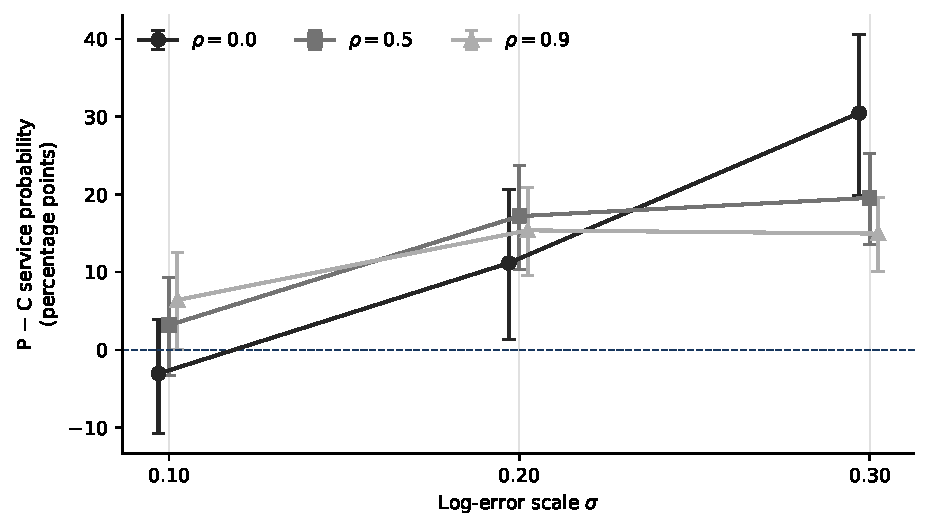
\includegraphics[width=\textwidth]{../paper/Fig1.pdf}
 \caption{Paired difference in service probability between the original
 procedure (P) and conservative speed (C) on the 46 common development
 instances, for fixed plans across the disturbance grid. Circles, squares and
 triangles mark $\rho=0$, $0.5$ and $0.9$; error bars are 95\% bootstrap
 intervals over instances, not simultaneous across cells.}
 \label{fig:reliability}
\end{figure}

\subsection{Capping the contraction}

Of the \FailureCount{} development instances on which the original procedure
admitted no plan, \CertifiedFailures{} met a certified reachability obstruction
at some buffer level. Capping (Table~\ref{tab:screen}) raised the number of admitted instances from
\OriginalSelected{} to \CappedSelected{} instances and pooled service by
\CappedGainInterval{} points. At 100 and 200 customers the capped procedure was
admitted on \CappedLargeSelected{} instances and pooled \CappedLargeRange\%. It
used \CappedDistanceCost\% more distance and \CappedFleetCost{} more vehicles
on average than the original procedure, rising to \CappedFleetLarge{} vehicles
at 200 customers.

\begin{table}[t]
\centering
\footnotesize
\setlength{\tabcolsep}{4pt}
\caption{Development study, all 53 instances. For each procedure: instances admitted by screening out of all instances of that size, with the number whose lower bound also reached 0.95 on the validation bank in parentheses, and pooled validated service probability (\%) with a 95\% bootstrap interval, fallback plans included.}
\label{tab:screen}
\begin{tabular}{@{}rllllll@{}}
\toprule
 & \multicolumn{2}{l}{Original procedure} & \multicolumn{2}{l}{Screened conservative} & \multicolumn{2}{l}{Capped procedure}\\
$n$ & Admitted & Pooled & Admitted & Pooled & Admitted & Pooled\\
\midrule
20 & 14/20 (14) & 81.6 [70.2, 91.9] & 15/20 (15) & 87.7 [79.0, 94.7] & 14/20 (14) & 81.6 [70.3, 92.0]\\
50 & 8/15 (8) & 72.7 [59.2, 86.4] & 4/15 (4) & 67.5 [58.2, 77.3] & 10/15 (10) & 80.1 [66.9, 90.8]\\
100 & 6/10 (5) & 81.3 [68.8, 93.3] & 4/10 (4) & 77.5 [67.2, 88.2] & 10/10 (9) & 97.5 [96.7, 98.2]\\
200 & 4/8 (3) & 80.6 [68.7, 92.3] & 2/8 (2) & 78.3 [71.0, 86.5] & 8/8 (7) & 97.6 [96.9, 98.2]\\
\bottomrule
\end{tabular}
\end{table}


The remaining shortfall comes from the fallback. Admitted plans averaged
\CappedSelectedMean\% validated service for the capped procedure, while its
\CappedFallbackCount{} fallback plans, all at 20 or 50 customers, averaged
\CappedFallbackMean\%. Of the admitted plans, \CappedRetained{} of
\CappedSelected{} kept a lower bound of at least 0.95 on the fresh validation
bank.

\subsection{Confirmatory evidence}

Table~\ref{tab:hypotheses} lists every prespecified hypothesis. In protocol~1
the original procedure exceeded conservative speed by \ConfHOneMean{} points and
capping added \ConfHTwoMean{}. Capping admitted \ConfHThreeK{} instances against
\ConfHThreeP{} and lost none. H2 and H3 are therefore not independent:
\HTwoFromKonly{} of the \ConfHTwoMean{} points of H2 come from the instances that
only the capped procedure admitted. The capped
procedure pooled \ConfPooledK\% over all instances, against \ConfPooledP\% for
the original procedure.

\begin{table}[!htbp]
\centering
\footnotesize
\caption{Every prespecified hypothesis of the three protocols. Primary hypotheses are marked $^{*}$. Differences are in percentage points of validated service-event probability unless stated; intervals are paired bootstrap intervals over instances (20,000 resamples), at 97.5\% for the two primary hypotheses of each study (Bonferroni) and 95\% otherwise. A hypothesis is confirmed when it meets the decision rule fixed in its protocol.}
\label{tab:hypotheses}
\begin{tabular}{@{}l>{\raggedright\arraybackslash}p{6.4cm}>{\raggedright\arraybackslash}p{3.0cm}ll@{}}
\toprule
Hyp. & Contrast & Estimate [interval] & Level & Decision\\
\midrule
\multicolumn{5}{@{}l}{\textit{Protocol 1: 53 new instances, OR-Tools generator}}\\
H1$^{*}$ & Original procedure minus conservative speed (\ConfCommon{} instances) & \ConfHOneMean{} [\ConfHOneLo, \ConfHOneHi] & 97.5\% & confirmed\\
H2$^{*}$ & Capped minus original procedure (\ConfInstances{} instances) & \ConfHTwoMean{} [\ConfHTwoLo, \ConfHTwoHi] & 97.5\% & confirmed\\
H3 & Instances admitted, capped versus original procedure & \ConfHThreeK{} vs \ConfHThreeP{} ($p=\ConfHThreeExact$) & exact & confirmed\\
H4 & Advantage over conservative speed at $\sigma=0.30$ minus at $\sigma=0.10$, $\rho=0$ & \ConfHFourMean{} [\ConfHFourLo, \ConfHFourHi] & 95\% & confirmed\\
\midrule
\multicolumn{5}{@{}l}{\textit{Protocol 2: 53 new instances, HGS and OR-Tools generators}}\\
G1$^{*}$ & HGS capped procedure minus HGS conservative speed (\CtwoCommon{} instances) & \CtwoGOneMean{} [\CtwoGOneLo, \CtwoGOneHi] & 97.5\% & confirmed\\
G2$^{*}$ & Conservative minus slack-aware fallback, OR-Tools capped procedure & \CtwoGTwoMean{} [\CtwoGTwoLo, \CtwoGTwoHi] & 97.5\% & not confirmed\\
G3 & The same for the uncapped OR-Tools procedure & \CtwoGThreeMean{} [\CtwoGThreeLo, \CtwoGThreeHi] & 95\% & confirmed\\
G4 & HGS minus OR-Tools capped procedure, both with conservative fallback & \CtwoGFourMean{} [\CtwoGFourLo, \CtwoGFourHi] & 95\% & estimate\\
\midrule
\multicolumn{5}{@{}l}{\textit{Protocol 3, part A: \PaInstances{} confirmatory instances with up to 100 customers}}\\
R1$^{*}$ & Screened robust with relief minus OR-Tools capped procedure & \PaROne{} [\PaROneLo, \PaROneHi] & 97.5\% & confirmed\\
R2$^{*}$ & Screened robust with relief minus HGS capped procedure (45 instances) & \PaRTwo{} [\PaRTwoLo, \PaRTwoHi] & 97.5\% & confirmed\\
R3 & The same contrast in vehicles & \PaRThree{} [\PaRThreeLo, \PaRThreeHi] & 95\% & confirmed\\
R4 & Distance (\%) of screened robust versus the most protective relieved setting & \PaRFour{} [\PaRFourLo, \PaRFourHi] & 95\% & confirmed\\
\midrule
\multicolumn{5}{@{}l}{\textit{Protocol 3, part B: \PbInstances{} new instances, best-screened fallback}}\\
F1$^{*}$ & Best-screened minus slack-aware fallback, OR-Tools capped procedure & \PbFOne{} [\PbFOneLo, \PbFOneHi] & 97.5\% & confirmed\\
F2$^{*}$ & Best-screened minus conservative fallback, HGS capped procedure & \PbFTwo{} [\PbFTwoLo, \PbFTwoHi] & 97.5\% & confirmed\\
F3 & Pooled service (\%), OR-Tools capped procedure with the new rule & \PbFThree{} [\PbFThreeLo, \PbFThreeHi] & 95\% & estimate\\
F4 & Pooled service (\%), HGS capped procedure with the new rule & \PbFFour{} [\PbFFourLo, \PbFFourHi] & 95\% & estimate\\
\bottomrule
\end{tabular}
\end{table}


Protocol~2 asked whether the gain survives a stronger generator. With HGS,
screening with capped contraction exceeded HGS conservative-speed planning by
\CtwoGOneMean{} points, and pooled service reached \CtwoPooledHGSK\% against
\CtwoPooledHGSCons\%. The HGS and OR-Tools capped procedures differed by
\CtwoGFourMean{} points, an interval that bounds the difference but, with no
equivalence margin set, does not show equivalence. Capping mattered more with
HGS: at 100 and 200 customers it raised admission from \CtwoHGSPAdmittedLarge{}
to \CtwoHGSKAdmittedLarge{} of \CtwoLarge{} instances. The conservative
fallback, suggested post hoc by protocol~1, did not measurably improve the
capped OR-Tools procedure (G2): that procedure fell back on only
\CtwoORTKFallbacks{} instances, and the new rule changed the plan on
\CtwoFallbacksChanged{} of them, with effects in both directions. It did help
the uncapped procedure (G3).

\subsection{Comparison with robust optimization}

On the \RobInstances{} development instances with up to 100 customers, the standard robust
model under box uncertainty had no plan on \RobNoPlanBoxSix{} instances at
$\theta=0.6$, each time because some customer could not be protected even on a
direct trip; every smaller budget failed on the same instances. With relief,
every setting had a plan, and the relieved settings traded distance for service
along a smooth frontier (Fig.~\ref{fig:robust}). Screened robust with relief
pooled \RobScreenedCapP\%, against \RobOrtCappedP\% for the OR-Tools and
\RobHgsCappedP\% for the HGS capped procedure, and used \RobScreenedCapMinusHgsFleet{}
more vehicles than the latter.

\begin{figure}[t]
 \centering
 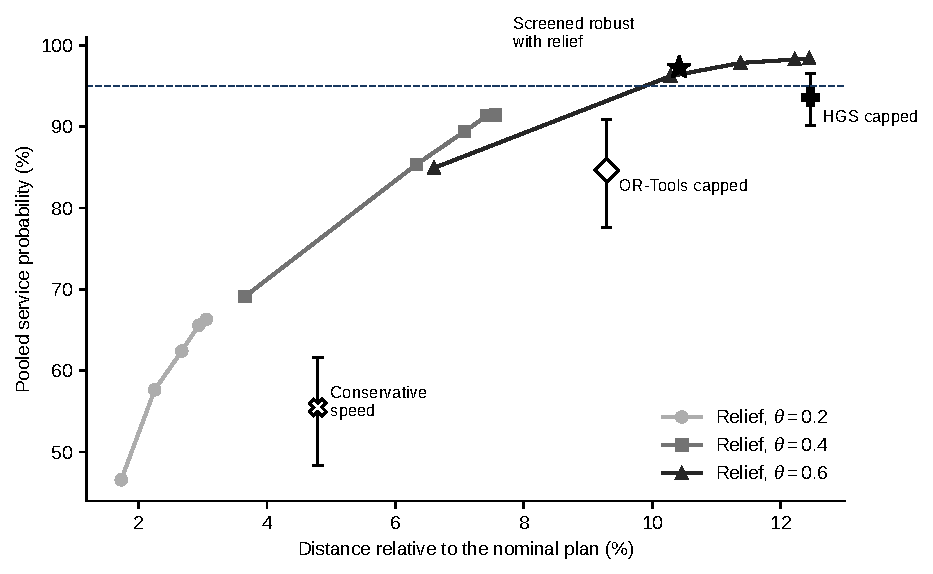
\includegraphics[width=\textwidth]{../paper/Fig2.pdf}
 \caption{Pooled validated service probability against mean distance relative
 to the nominal robust plan, on the 45 development instances with up to 100
 customers. Lines join the relieved robust settings for each $\theta$, from
 $\Gamma=1$ to box uncertainty; the screened procedures and conservative speed
 are shown with 95\% bootstrap intervals. The dashed line marks the target.}
 \label{fig:robust}
\end{figure}

Part A of protocol~3 confirmed this on the confirmatory instances with up to 100
customers. Screened robust with relief exceeded the OR-Tools capped procedure by
\PaROne{} points over all \PaInstances{} of them, and the HGS capped procedure by
\PaRTwo{} points over the 45 of protocol~2, where HGS plans exist; the two
estimates agree only by coincidence. It
pooled \PaScreenedP\% and used \PaRThree{} more vehicles than the HGS
procedure. Within the robust family, screening returned plans \PaRFourAbs\%
shorter than the most protective setting for \PaBoxMinusScr{} points less
service. When the robust plans were restricted, after the fact, to no more
vehicles than the comparator's plan, they were not measurably more reliable:
the differences were \FmConfHgs{} [\FmConfHgsLo, \FmConfHgsHi] points against
the HGS and \FmConfOrt{} [\FmConfOrtLo, \FmConfOrtHi] against the OR-Tools
capped procedure. On these instances the screened procedures trade some
reliability for fewer vehicles, returning the shortest candidate that passes a
stated test. Runs with 200 customers are reported in \SI{sec:robust}.

\subsection{Fallback rule}

After the first two protocols, the stored records showed that returning the
best-screened candidate when nothing is admitted raised pooled service in every
study and procedure, by \FbGainMin{} to \FbGainMax{} points. Part B of
protocol~3 tested the rule on \PbInstances{} new instances. Over each procedure's
default fallback, it improved the OR-Tools capped procedure by \PbFOne{} points
and the HGS capped procedure by \PbFTwo{}, to pooled service of \PbFThree\% and
\PbFFour\%. Both estimates stay just below the 95\% target. On \PbNoAnchor{}
instance the anchor solves found no plan, so neither procedure could run and it
scored zero; without it, pooled service was \PbExOrt\% and \PbExHgs\%
(descriptive). Plans returned by the fallback have not passed the screen.

\subsection{Sensitivity and further checks}\label{sec:checks}

\emph{Objective weights.} On the development instances, equal weights admitted
fewer instances (\WtEqualAdmitted{} against \WtBaseAdmitted{} in the same run)
and cut the advantage over conservative speed to \WtEqualPCMean{} points
[\WtEqualPCLo, \WtEqualPCHi]. A later run on another machine, repeating both
vectors, cut it from \BrOrigAdv{} to \BrEqAdv{} points [\BrEqAdvLo, \BrEqAdvHi]. Raising the driver-duration weight alone changed
service by \BrDurDiff{} points and raising the fleet weight alone by
\BrFleetDiff{}, so the advantage depends on how much waiting time the objective
leaves to absorb delay. No protocol varied the weights (\SI{sec:weights}).

\emph{Benchmark instances.} On \SolomonN{} Solomon R1 and RC1 instances, OR-Tools
found a plan for \SolomonPlans{} and screening admitted \SolomonAdmitted{}. With
HGS on 20 Gehring--Homberger instances with 200 customers \citep{gehring1999},
the procedure could run on \GhAttempted{}, admitted \GhAdmitted{}, and exceeded
conservative speed by \GhDiff{} points [\GhDiffLo, \GhDiffHi]
(Sections~\ref{S-sec:solomon} and~\ref{S-sec:gh}).

\emph{Delay-model misspecification.} Under four alternative delay models, the
fixed plans of the capped procedures lost up to \MisCappedDrop{} points and
their advantage over conservative speed held. Screening the stored candidates
again under each model, with the best-screened fallback, kept pooled service
between \ResLoOrt{} and \ResHiHgs\% (\SI{sec:misspec}).

\emph{Family-wise screening and computation time.} Over all studies and
procedures, a Bonferroni bound over the 13 buffer levels removed all
\FwMissOrig{} of the \FwAdmittedOrig{} admitted plans that later missed the
validation bound, while \FwMissFw{} newly selected plan missed it, at the cost of at most \FwLostMax{} admissions per study and
procedure and between \FwPooledChangeMin{} and \FwPooledChangeMax{} points of
pooled service. Screening a candidate took \TimeScreenTwenty{} to
\TimeScreenTwoHundred{}~ms, against seconds to generate it
(\SI{sec:familywise}).

\section{Discussion and limitations}\label{sec:discussion}

For a planner who already uses a VRPTW solver, the results suggest a practical
change. Generating a handful of buffered variants and screening them on
simulated days costs little beyond the solves, needs no change to the solver or
its objective, and replaced a fixed 20\% pad with plans that were measurably
more reliable on the same instances. Each admitted plan has a tested lower
bound on a defined service event, and the validation bank reports how that plan
behaved on days it had not seen. The
reachability cap is a one-line change that removed most certified failures and
should be used with any buffer-based method, robust models included.

The evidence has clear limits. The instances are synthetic and the disturbance
parameters are assumed; they have not been calibrated to vehicle GPS data, so
the numbers are not forecasts for a real fleet. The protocols test
repeatability within one generator and one delay model, and the Solomon and
Gehring--Homberger checks are small. The OR-Tools generator is weaker than the
state of the art, which is why protocol~2 repeated the test with HGS; two
generators still do not show that the result holds for every solver. The robust
comparison covers one budgeted model with one search configuration, and the
distributionally robust and riskiness-index methods
\citep{jaillet2016,zhang2019} are not compared. The advantage depends on the
objective weights, and equal weights more than halved it. The Wilson bound is a
per-candidate guarantee, not a simultaneous one over the grid. Finally, the
evaluation keeps every departure fixed and excludes breakdowns, new orders and
rolling-horizon replanning, so it is stricter than an operator who adjusts
departures would face, and it says nothing about recovery once a delay occurs.

Under the prespecified fallback rules, pooled service stayed below 95\% in
every study because of instances on which nothing was admitted. The best-screened fallback narrows the gap, but closing it
needs better candidates on those instances, which is where a stronger or
stochastic generator could add most.

\section{Conclusion}\label{sec:conclusion}

Screening a family of buffered plans from a standard VRPTW solver gave more
reliable service than uniform travel-time padding on matched synthetic
instances, with OR-Tools and with HGS, and three timestamped protocols supported
the main findings. One primary hypothesis was not confirmed: returning the
conservative-speed plan when nothing is admitted did not measurably help the
capped OR-Tools procedure, while returning the best-screened candidate did.
Capping each customer's buffer at its direct-reachability limit removed a
failure that also stops robust models from finding any plan. A budgeted-robust
optimizer with that relief was more reliable still, but used more vehicles, and
its advantage was not measurable at the comparator's fleet size. The screening
layer and the reachability relief worked with every planner tested.
Calibrated delay data and real road networks are the next test.

\section*{Data availability}
All code, generated instances, raw records and analysis scripts are openly
available on Zenodo \citep{ali2026archive}; code is released under the MIT
License and records under CC BY 4.0. The three protocol freezes are separate
Zenodo records \citep{ali2026freeze,ali2026freeze2,ali2026freeze3}. The Solomon
and Gehring--Homberger instance files are third-party data
\citep{solomon1987,ml4vrp2024,gehring1999} and remain under their original
terms.

\section*{Use of generative AI}
Generative AI assistants (OpenAI's ChatGPT and Anthropic's Claude) were used for
code development, code review, checking the analysis, and drafting and editing
text. They are not authors. Every experiment was run from the archived code and
every reported number regenerates from the archived records. The author reviewed
all code and text and takes full responsibility for the content.

\section*{Acknowledgements}
The author thanks the researchers who answered methodological questions by
e-mail during the project. All claims in the paper rest on the reported model,
code and experiments.

\bibliographystyle{itor}
\bibliography{../paper/sn-bibliography}

\end{document}
